\documentclass[a4paper,12pt]{report}

%Русский язык
\usepackage[T2A]{fontenc}
\usepackage[utf8]{inputenc}
\usepackage[english,russian]{babel}
\usepackage{cmap}

%Работа с кодом
\usepackage{listings}
\usepackage{color}

\definecolor{green}{rgb}{0,0.6,0}
\definecolor{gray}{rgb}{0.5,0.5,0.5}
\definecolor{red}{rgb}{0.6,0,0}

\lstset{
        language=Python, 
        basicstyle=\small\ttfamily, 
        numberstyle=\tiny,           
        columns=flexible,
        stepnumber=1,                   
        numbersep=5pt,        
        showspaces=false,
        showstringspaces=false,
        showtabs=false,
        tabsize=2,                
        captionpos=b,              
        breaklines=true,           
        breakatwhitespace=false,
        keywordstyle=\color{green},
        commentstyle=\color{gray},
        stringstyle=\color{red},      
}

%Математика
\usepackage{amsmath,amsfonts,amssymb,amsthm,mathtools} 

%Изображения
\usepackage{float}
\usepackage{graphicx}
\graphicspath{ {./img/} }

%Поля страницы
\usepackage{geometry} 
\geometry{left=2.3cm} 
\geometry{right=1.8cm} 
\geometry{top=2cm} 
\geometry{bottom=2.5cm} 

%Отступы
\usepackage{indentfirst}
\setlength{\parskip}{0cm}

\begin{document} 

\begin{titlepage}
\newpage
	\begin{center}
		\large Санкт-Петербургский политехнический университет Петра Великого\\
		Институт компьютерных наук и технологий\\
		Высшая школа интеллектуальных систем и суперкомпьютерных технологий\\
	\end{center}
\vspace{7cm}

\begin{center}
		\large \textbf{Отчёт по лабораторной работе №3} \\
		\textbf{Дисциплина:} Телекоммуникационные технологии\\
		\textbf{Тема:} Апериодические сигналы
\end{center}
\vspace{4cm}
	
\begin{flushright}
		\large Работу выполнил:\\ Ляшенко В.В.\\
		Группа: 3530901/80201\\
		Преподаватель:\\ Богач Н.В.
\end{flushright}

\vspace{\fill}
\begin{center}
	\large Санкт-Петербург\\ 2021
	\end{center}
\end{titlepage}

\tableofcontents
\listoffigures
\lstlistoflistings

\chapter{Упражнение 3.1}
    В начале нам требуется загрузить и послушать примеры из блокнота \texttt{chap03.ipynb}.
    
    Теперь в примере с утечкой заменим окно Хэмминга одним из окон, предоставляемых NumPy, и посмотрим как они влияют на утечку. Утечка при использовании окна Хэмминга имеет вид, представленный на Рис.1.1.
\begin{figure}[H]
        \centering
        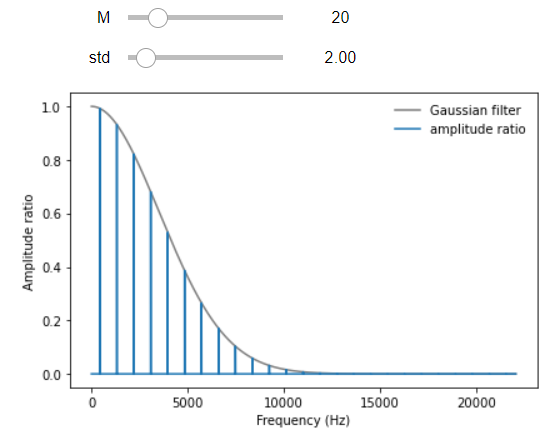
\includegraphics[width=0.8\textwidth]{fig1-1.PNG}
        \caption{Утечка. Окно Хэмминга}
        \label{fig:fig1-1}
\end{figure}

    NumPy дает функции для вычисления других оконных функций, такие как \texttt{bartlett}, \texttt{blackman}, \texttt{hanning} и \texttt{kaiser}. Используем их (Рис.1.2).
\begin{lstlisting}[caption=Вычисление разных оконных функций]
       import thinkplot
       import numpy as np
       
       wave = signal.make_wave(duration)
       wave.window(np.bartlett(len(wave)))
       spectrum = wave.make_spectrum()
       spectrum.plot(high=880, label="bartlett")

       wave = signal.make_wave(duration)
       wave.window(np.blackman(len(wave)))
       spectrum = wave.make_spectrum()
       spectrum.plot(high=880, label="blackman")

       wave = signal.make_wave(duration)
       wave.window(np.hanning(len(wave)))
       spectrum = wave.make_spectrum()
       spectrum.plot(high=880, label="hanning")

       wave = signal.make_wave(duration)
       wave.window(np.kaiser(len(wave),5))
       spectrum = wave.make_spectrum()
       spectrum.plot(high=880, label="kaiser")

       thinkplot.config(xlabel='Frequency (Hz)', legend=True)
\end{lstlisting}
\begin{figure}[H]
        \centering
        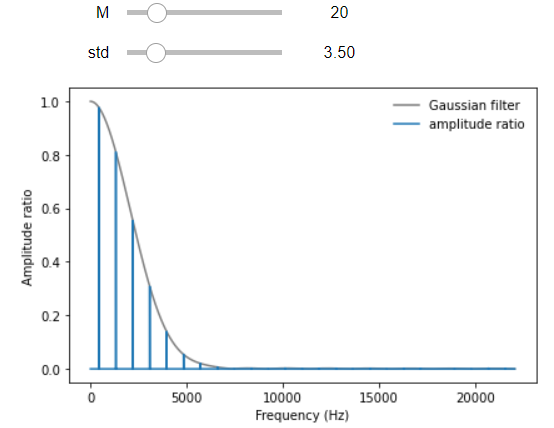
\includegraphics[width=0.8\textwidth]{fig1-2.PNG}
        \caption{Применение разных окон}
        \label{fig:fig1-2}
\end{figure}
    
    Все окна хорошо справляются с уменьшением утечки.
    
\chapter{Упражнение 3.2}
\section{Класс SawtoothChirp}
    Напишем класс \texttt{SawtoothChirp}, расширяющий \texttt{Chirp} и переопределяющий \texttt{evaluate} для генерации пилообразного сигнала с линейно увеличивающейся частотой.
\begin{lstlisting}[caption=Класс SawtoothChirp]
from thinkdsp import Chirp, normalize, unbias, PI2

class SawtoothChirp(Chirp):

    def evaluate(self, ts):
        freqs = np.linspace(self.start, self.end, len(ts))
        dts = np.diff(ts, prepend=0)
        dphis = PI2 * freqs * dts
        phases = np.cumsum(dphis)
        cycles = phases / PI2
        frac, _ = np.modf(cycles)
        ys =  normalize(unbias(frac), self.amp)
        return ys
\end{lstlisting}
\section{Спектрограмма}
    Нарисуем эскиз спектрограммы этого сигнала, а затем распечатаем. 
\begin{lstlisting}[caption=Создание спектрограммы]
       signal = SawtoothChirp(start=220, end=880)
       wave = signal.make_wave(duration=1, framerate=4000)
       spectrogram = wave.make_spectrogram(128)
       spectrogram.plot()
       decorate(xlabel='Time (s)', ylabel='Frequency (Hz)')
\end{lstlisting}
\begin{figure}[H]
        \centering
        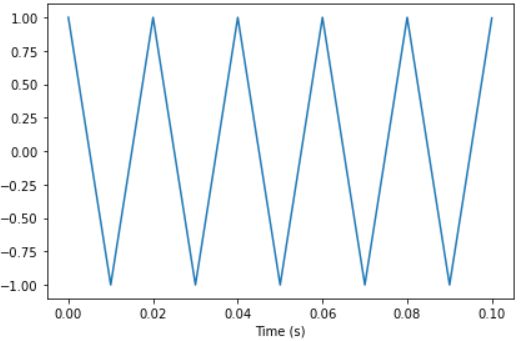
\includegraphics[width=0.8\textwidth]{fig2-1.PNG}
        \caption{Спектрограмма}
        \label{fig:fig2-1}
\end{figure}
    
    Мы можем увидеть на рис.2.1, как гармоники с наложенными частотами отражаются от частоты сворачивания. 
    
    Послушаем получившийся сигнал.  
    Именно отрожающиеся гармоники мы слышим как фоновое шипение.     
    
\chapter{Упражнение 3.3}
    Создадим пилообразный чирп, меняющийся от 2500 до 3000 Гц, и на его основе сгенерируем сигнал длительностью 1 с и частотой кадров 20 кГц. 
\begin{lstlisting}[caption=Создание пилообразного чирпа]
       signal = SawtoothChirp(start=2500, end=3000)
       wave = signal.make_wave(duration=1, framerate=20000)
\end{lstlisting}
    
    Теперь нам нужно вывести спектр данного сигнала. Но прежде мы должны предположить как он будет выглядеть. Так как основная частота меняется в диапазоне от 2500 до 3000 Гц, то здесь будет большой всплеск. На первой гармоники (диапазон от 5000 до 6000 Гц,) будет всплеск поменьше, а на второй гармоники ([7500;9000]) - ещё ниже. 
    Выведем спектр.
\begin{lstlisting}[caption=Получение спектра чирпа]
       spectrogram = wave.make_spectrogram(128)
       spectrogram.plot()
       decorate(xlabel='Time (s)', ylabel='Frequency (Hz)')
\end{lstlisting}
\begin{figure}[H]
        \centering
        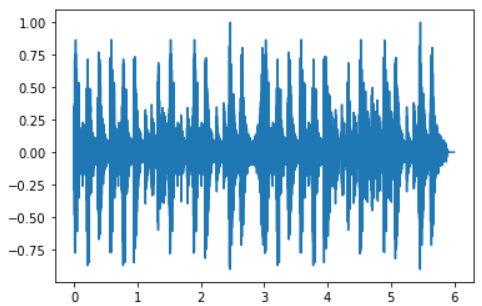
\includegraphics[width=0.8\textwidth]{fig3-1.PNG}
        \caption{Спектр чирпа}
        \label{fig:fig3-1}
\end{figure}

    Как мы можем видеть из рис.3.1 полученный спектр совпал с ожидаемым.
    
\chapter{Упражнение 3.4}
    В данном упражнении нам необходимо распечатать спектрограмму первых нескольких секунд звука глиссандо. Воспользуемся подсказкой из пособия и скачаем произведение "Rhapsody in Blue" Джорджа Гершвина, которое содержит глиссандо.
\begin{lstlisting}[caption=Получение звука глиссандо]
       from thinkdsp import read_wave
       wave = read_wave('sounds/rhapblue11924.wav')
       segment = wave.segment(start=2, duration=9)
       segment.make_audio()
\end{lstlisting}
    Теперь выведем его спектрограмму (Рис.4.1).
\begin{lstlisting}[caption=Получение спектрограммы]
       spectrogram = segment.make_spectrogram(512)
       spectrogram.plot()
       decorate(xlabel='Time (s)', ylabel='Frequency (Hz)')
\end{lstlisting}
\begin{figure}[H]
        \centering
        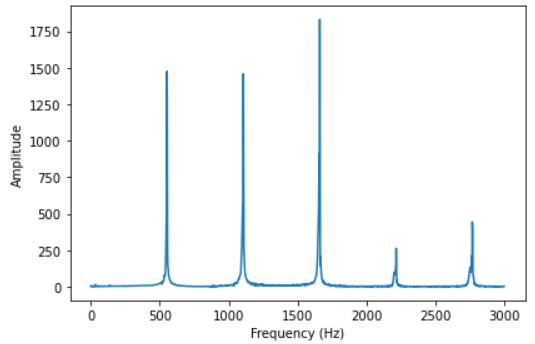
\includegraphics[width=0.8\textwidth]{fig4-1.PNG}
        \caption{Спектрограмма глиссандо}
        \label{fig:fig4-1}
\end{figure}

\chapter{Упражнение 3.5}
\section{Класс TromboneGliss}
    Напишем класс \texttt{TromboneGliss}, расширяющий \texttt{Chirp} и предоставляющий \texttt{evaluate}.
\begin{lstlisting}[caption=Класс TromboneCliss]
class TrombonGliss(Chirp):
    
    def evaluate(self, ts):
        start, end = 1.0 / self.start, 1.0 / self.end
        freqs = 1.0 / np.linspace(start, end, len(ts))
        
        dts = np.diff(ts, prepend=0)
        dphis = PI2 * freqs * dts
        phases = np.cumsum(dphis)
        ys = self.amp * np.cos(phases)
        return ys
\end{lstlisting}
    
    Создадим сигнал, имитирующий глиссандо на тромбоне от C3 до F3, и обратно до C3. C3 - 262 Гц, F3 - 349 Гц.
\begin{lstlisting}[caption=Создание сигнала]
       C3 = 262
       F3 = 349
       signal = TromboneGliss(C3, F3)
       wave_CF = signal.make_wave(duration=1)
       wave_CF.apodize()
       signal = TromboneGliss(F3, C3)
       wave_FC = signal.make_wave(duration=1)
       wave_FC.apodize()
       wave = wave_CF | wave_FC
       wave.make_audio()
\end{lstlisting}    
\section{Спектрограмма}
       Напечатаем спектрограмму полученного сигнала.
\begin{lstlisting}[caption=Получение спектрограммы]
       spectrogram = wave.make_spectrogram(1024)
       spectrogram.plot(high=1000)
       decorate(xlabel='Time (s)', ylabel='Frequency (Hz)')
\end{lstlisting}
\begin{figure}[H]
        \centering
        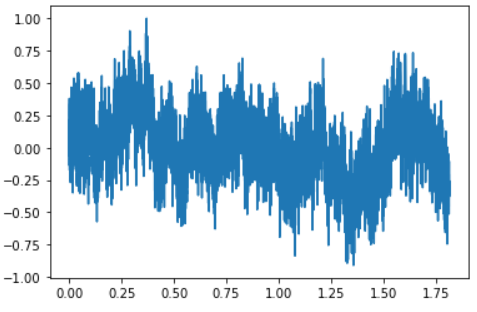
\includegraphics[width=0.8\textwidth]{fig5-1.PNG}
        \caption{Спектрограмма глиссандо C3-F3}
        \label{fig:fig5-1}
\end{figure}
    
    Как мы можем видеть на рис.5.1, глиссандо больше похоже на линейный чирп.

\chapter{Упражнение 3.6}
\section{Спектрограмма}
    Скачаем с \texttt{https://freesound.org} запись серии гласных звуков и посмотрим на спектрограмму.
\begin{lstlisting}[caption=Получение спектрограммы гласных звуков]
       wave = read_wave('sounds/523079__team-saul-nosthas__vowels-of-various-people.wav')
       vowels = wave.segment(start=0, duration=6)
       vowels.make_spectrogram(512).plot(high=1500)
       decorate(xlabel='Time (s)', ylabel='Frequency (Hz)')
       vowels.make_audio()
\end{lstlisting}
\begin{figure}[H]
        \centering
        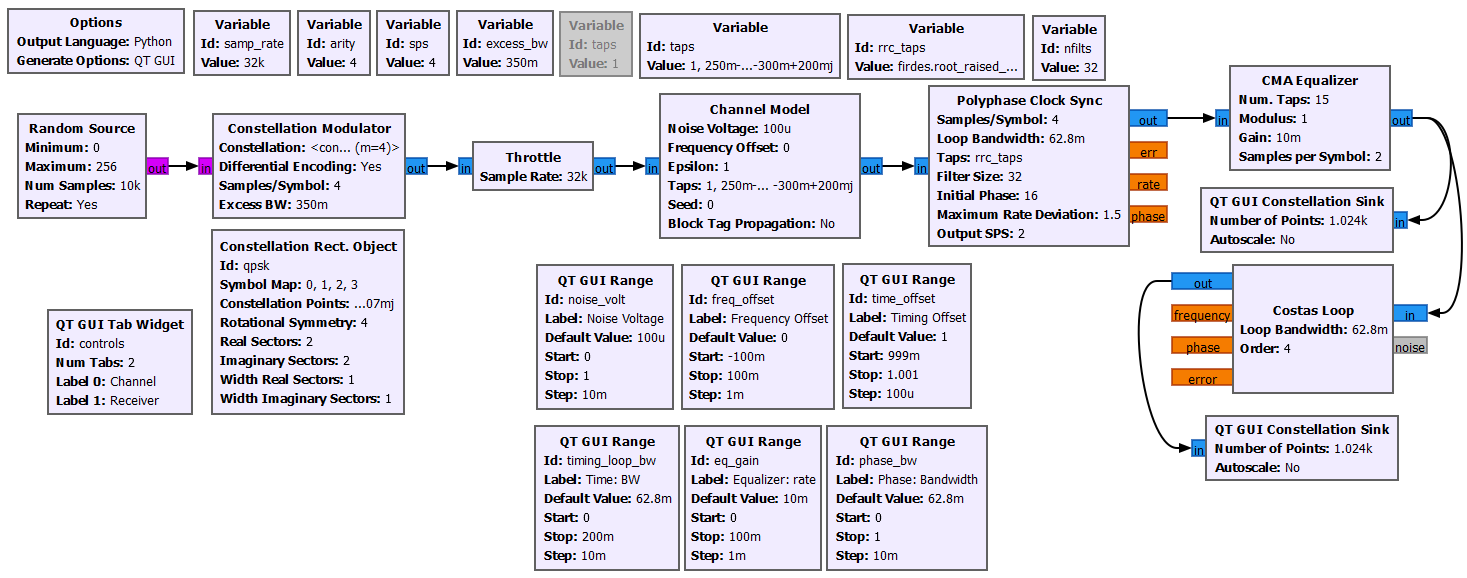
\includegraphics[width=0.8\textwidth]{fig6-1.PNG}
        \caption{Спектрограмма гласных звуков}
        \label{fig:fig6-1}
\end{figure}

    Как мы можем видеть на рис.6.1, разные гласные звуки имеют разные частоты, так что различить гласные по спектру возможно, но очень трудно.
\section{Спектры гласных звуков}
    Пики на спектрограмме называются формантами. Гласные звуки различаются соотношением амплитуд первых двух формант относительно основного тона.

    Посмотрим на спектры каждого звука.

\subsection{Звук а}
\begin{lstlisting}[caption=Получение спектра звука а]
       segment = vowels.segment(start=0.5, duration=0.75)
       segment.make_spectrum().plot(high=1000)
       decorate(xlabel='Frequency (Hz)')
\end{lstlisting}
\begin{figure}[H]
        \centering
        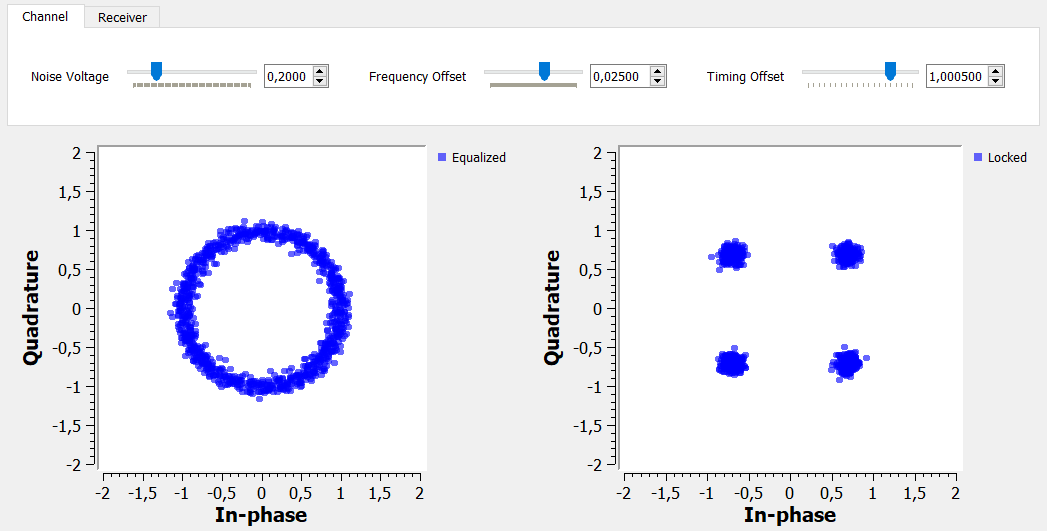
\includegraphics[width=0.8\textwidth]{fig6-2.PNG}
        \caption{Спектр звука а}
        \label{fig:fig6-2}
\end{figure}

    На рис.6.2 видно, что основная частота находится между 200 и 300 Гц. Следующие самые высокие пики находятся между 500-600 Гц и 700-800 Гц соответственно.

\subsection{Звук э}
\begin{lstlisting}[caption=Получение спектра звука э]
       segment = vowels.segment(start=1.5, duration=0.9)
       segment.make_spectrum().plot(high=1000)
       decorate(xlabel='Frequency (Hz)')
\end{lstlisting}
\begin{figure}[H]
        \centering
        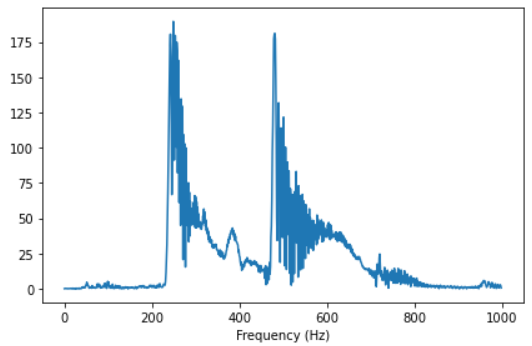
\includegraphics[width=0.8\textwidth]{fig6-3.PNG}
        \caption{Спектр звука э}
        \label{fig:fig6-3}
\end{figure}
    На рис.6.3 мы видим два похожих пика на 300 и 500 Гц соответственно.

\subsection{Звук и}
\begin{lstlisting}[caption=Получение спектра звука и]
       segment = vowels.segment(start=2.7, duration=0.7)
       segment.make_spectrum().plot(high=1000)
       decorate(xlabel='Frequency (Hz)')
\end{lstlisting}
\begin{figure}[H]
        \centering
        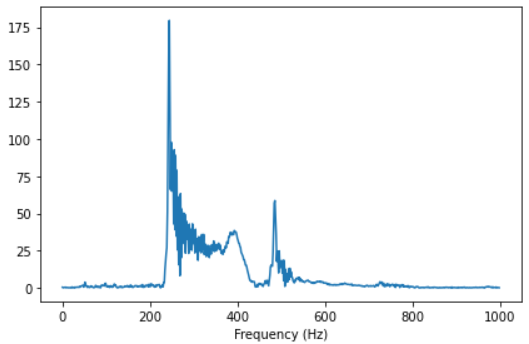
\includegraphics[width=0.8\textwidth]{fig6-4.PNG}
        \caption{Спектр звука и}
        \label{fig:fig6-4}
\end{figure}

    На рис.6.4 мы видим основную частоту на 200, а следующий пик на 500 Гц.

\subsection{Звук о}
\begin{lstlisting}[caption=Получение спектра звука о]
       segment = vowels.segment(start=3.6, duration=0.8)
       segment.make_spectrum().plot(high=1000)
       decorate(xlabel='Frequency (Hz)')
\end{lstlisting}
\begin{figure}[H]
        \centering
        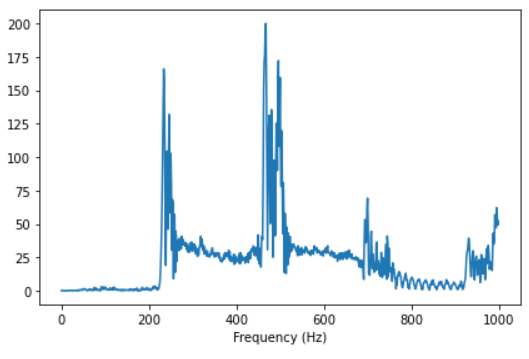
\includegraphics[width=0.8\textwidth]{fig6-5.PNG}
        \caption{Спектр звука о}
        \label{fig:fig6-5}
\end{figure}

    Звук о имеет высокоамплитудную форманту около 500 Гц, даже выше основной частоты.

\subsection{Звук у}
\begin{lstlisting}[caption=Получение спектра звука у]
       segment = vowels.segment(start=4.5, duration=0.6)
       segment.make_spectrum().plot(high=1000)
       decorate(xlabel='Frequency (Hz)')
\end{lstlisting}
\begin{figure}[H]
        \centering
        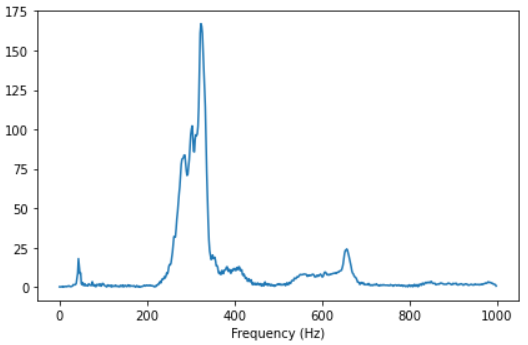
\includegraphics[width=0.8\textwidth]{fig6-6.PNG}
        \caption{Спектр звука у}
        \label{fig:fig6-6}
\end{figure}

    Звук у имеет высокоамплитудную форманту около 300 Гц и не имеет высокочастотных составляющих.
\chapter{Выводы}
    В результате выполнения данный работы мы познакомились с понятиями апериодических сигналов, частотные компоненты которых изменяются во времени. К ним относятся практически все сигналы. А также с чирпами - сигналами с переменной частотой.
    
    Кроме того, мы научились работать со спектрограммами и окнами. 
    
    Спектрограмма - это способ визуализации кратковременных ПФ. У неё на оси $x$ время, а на оси $y$ частоты.
    
    Окно - это функция, преобразующая апериодический сегмент во нечто похожее на периодическое.   
\end{document}